\documentclass[conference]{IEEEtran}
\IEEEoverridecommandlockouts

\usepackage{cite}
\usepackage{amsmath,amssymb,amsfonts}
\usepackage{algorithmic}
\usepackage{graphicx}
\usepackage{textcomp}
\usepackage{xcolor}
\usepackage{booktabs}
\usepackage{url}
\usepackage{microtype}

\def\BibTeX{{\rm B\kern-.05em{\sc i\kern-.025em b}\kern-.08em
    T\kern-.1667em\lower.7ex\hbox{E}\kern-.125emX}}

\begin{document}

\title{A 20-Gb/s 61.7-dB$\Omega$ SiGe-BiCMOS Optical Transimpedance Amplifier with Active DC-Offset Cancellation in Open-Source 130-nm IHP SG13G2\\
\thanks{This work was submitted to the SMACD 2027 Open-Source Design Challenge. Fabricated via the Chips JU ODE4EC-AMS project.}
}

\author{\IEEEauthorblockN{Open Silicon Design Team}
\IEEEauthorblockA{\textit{SMACD 2027 Open-Source Design Challenge Initiative} \\
Public Repository: \url{https://github.com/anonymous-smacd/sg13g2-optical-tia}}
}

\maketitle

\begin{abstract}
We present a high-speed, fully open-source 20-Gb/s optical receiver front-end designed in the open-source IHP SG13G2 130-nm SiGe BiCMOS technology ($f_T = 300$~GHz, $f_{\max} = 500$~GHz). The circuit comprises an optimized shunt-feedback transimpedance amplifier (SF-TIA) core, an active DC-offset cancellation (DCOC) servo loop capable of compensating up to 2~mA of unipolar photodiode current, and a 50-$\Omega$ back-terminated current-mode logic (CML) output driver. By leveraging the ultra-high transconductance and low base resistance of SiGe heterojunction bipolar transistors (HBTs), the front-end achieves a -3-dB transimpedance bandwidth of 20.5~GHz, a mid-band transimpedance gain of 61.7~dB$\Omega$ ($1.22~\text{k}\Omega$), an average input-referred noise current density of $3.87~\text{pA}/\sqrt{\text{Hz}}$, and an integrated input RMS noise of $0.57~\mu\text{A}$, yielding a calculated optical sensitivity of $-23.2$~dBm at a bit error rate of $10^{-12}$. Large-signal transient simulations with a 20-Gb/s PRBS-7 data stream demonstrate a wide eye opening of $245~\text{mV}_{\text{pp}}$ with an RMS jitter of $1.15$~ps. The design was synthesized, laid out, and physically verified end-to-end using strictly open-source EDA tools (Xschem, Ngspice, and KLayout). The core die area occupies $0.48~\text{mm}^2$ including RF ground-signal-ground (GSG) pads, and passes 100\% DRC and LVS checks against official foundry decks.
\end{abstract}

\begin{IEEEkeywords}
Transimpedance amplifier (TIA), SiGe BiCMOS, IHP SG13G2, optical receiver, open-source EDA, active DC-offset cancellation, eye diagram.
\end{IEEEkeywords}

\section{Introduction}
High-speed optical interconnects are the cornerstone of contemporary data centers, high-performance computing (HPC) clusters, and telecommunication backbones. As data rates per lane surpass 10 to 25~Gb/s, the design of low-noise, wide-bandwidth optical receiver analog front-ends faces stringent trade-offs governed by the transimpedance gain-bandwidth-noise limit \cite{razavi_rf, sackinger}. 

Historically, achieving tens of gigahertz bandwidth with sub-$10~\text{pA}/\sqrt{\text{Hz}}$ input noise required proprietary sub-100-nm CMOS or high-cost III-V processes using closed-source, commercial EDA suites. However, the release of the open-source IHP SG13G2 130-nm SiGe BiCMOS process development kit (PDK) has dramatically shifted this paradigm \cite{ihp_pdk}. Featuring high-performance SiGe:C Heterojunction Bipolar Transistors (HBTs) with cutoff frequencies $f_T = 300$~GHz and $f_{\max} = 500$~GHz alongside a 1.2-V/3.3-V CMOS baseline, SG13G2 offers exceptional transconductance per unit current ($g_m / I_C = 1/V_T \approx 38.7~\text{V}^{-1}$) and minimal base parasitic resistance ($r_b < 10~\Omega$).

In this work, we present a complete, tapeout-ready 20-Gb/s optical transimpedance amplifier front-end targeting the SMACD 2027 Open-Source Design Challenge. The key contributions of this work are:
\begin{enumerate}
    \item A high-performance SiGe-BiCMOS TIA topology incorporating a shunt-feedback core with capacitive peaking, achieving a 20.5-GHz bandwidth and 61.7-dB$\Omega$ transimpedance gain.
    \item An integrated active DCOC servo loop using a sub-threshold CMOS operational transconductance amplifier (OTA) and high-$Q$ on-chip MIM capacitors to suppress DC baseline wander without external AC-coupling passives.
    \item A completely open-source, fully reproducible design methodology executed with Xschem, Ngspice, and KLayout, validated through automated CI workflows and verified clean against official IHP DRC and LVS decks.
\end{enumerate}

\section{Circuit Architecture and Sizing}

\subsection{Top-Level Architecture}
The block diagram of the proposed optical front-end is depicted in Fig.~\ref{fig:schematic}. The front-end interfaces with a high-speed PIN photodiode modeled with a junction capacitance $C_{\text{PD}} = 40$~fF and a series resistance $R_s = 10~\Omega$. The architecture comprises: (i) an input ESD protection cell and RF GSG pad; (ii) the main shunt-feedback TIA core; (iii) a symmetric dummy replica TIA stage; (iv) an active DCOC servo integrator; and (v) a 50-$\Omega$ back-terminated differential CML output driver.

\subsection{Shunt-Feedback TIA Core Design}
The core TIA adopts a common-emitter (CE) input transistor ($Q_1$, npn13G2) cascaded with an emitter-follower buffer ($Q_2$, npn13G2). The feedback resistor $R_F$ establishes the transimpedance gain while setting the input impedance to:
\begin{equation}
R_{\text{in}} = \frac{R_F}{1 + A_0}
\end{equation}
where $A_0 = g_{m1} (R_{C1} \parallel r_{\pi 2})$ represents the open-loop voltage gain of the forward amplifier. To maximize $f_T$, $Q_1$ is biased at $I_{C1} = 2.5$~mA ($N_x = 2$ emitter fingers, $W_e = 0.12~\mu\text{m}$, $L_e = 0.96~\mu\text{m}$), yielding $g_{m1} = 96.7$~mS and $r_{b1} = 9.0~\Omega$. With $R_{C1} = 300~\Omega$, an open-loop gain $A_0 \approx 28$ is realized, lowering the closed-loop input resistance to $R_{\text{in}} \approx 42~\Omega$. Consequently, the dominant input pole is pushed well beyond the operating Nyquist frequency:
\begin{equation}
\omega_{p,\text{in}} \approx \frac{1 + A_0}{R_F (C_{\text{PD}} + C_{\text{pad}} + C_{\pi 1} + (1+A_0)C_{\mu 1})}
\end{equation}

A small metal-insulator-metal (MIM) peaking capacitor $C_F = 20$~fF is placed in parallel with $R_F$. This introduces a left-half-plane zero $z_F = 1/(R_F C_F)$, neutralizing the second pole created by the emitter follower and extending the -3-dB bandwidth to 20.5~GHz with Butterworth maximally-flat response.

\subsection{Noise Optimization}
The equivalent input-referred noise current spectral density of the SiGe HBT TIA is formulated as:
\begin{equation}
\overline{i_{n,\text{in}}^2} = \frac{4k_B T}{R_F} + 2q I_{B1} + \frac{2q I_{C1} + 4k_B T r_{b1} g_{m1}^2}{g_{m1}^2} \left[ \frac{1}{R_F^2} + \omega^2 C_{\text{in}}^2 \right]
\end{equation}
At low-to-mid frequencies, thermal noise from $R_F$ ($3.64~\text{pA}/\sqrt{\text{Hz}}$) and base shot noise $2q I_B$ ($0.94~\text{pA}/\sqrt{\text{Hz}}$) dominate. At high frequencies, collector shot noise and base resistance thermal noise transferred by $\omega C_{\text{in}} / g_{m1}$ cause the noise density to rise quadratically. Thanks to the ultra-low $r_b$ and high $\beta \approx 900$ of the SG13G2 HBTs, the average input noise density across 1--10~GHz is held to just $3.87~\text{pA}/\sqrt{\text{Hz}}$. Integrating over the 20.5-GHz band yields a total input RMS noise current:
\begin{equation}
I_{n,\text{rms}} = \sqrt{\int_0^{B} \overline{i_{n,\text{in}}^2}(f) df} = 0.57~\mu\text{A}
\end{equation}
Assuming a standard photodiode responsivity $\mathcal{R} = 0.85$~A/W, the optical sensitivity for a bit error rate $\text{BER} = 10^{-12}$ ($Q = 7.03$) is calculated as:
\begin{equation}
P_{\text{sens}} = 10 \log_{10} \left( \frac{Q \cdot I_{n,\text{rms}}}{\mathcal{R} \cdot 1~\text{mW}} \right) = -23.2~\text{dBm}
\end{equation}

\subsection{Active DC-Offset Cancellation (DCOC) Loop}
Unipolar optical signals introduce a significant DC current component $I_{\text{DC}} = 0.5 I_{\text{pp}} + I_{\text{dark}}$. Without offset removal, this current shifts the base bias of $Q_1$, driving the amplifier into saturation. To eliminate off-chip AC-coupling capacitors, an active DCOC loop is implemented. 

The servo loop senses the differential error between the main TIA output and a dummy replica TIA stage using a PMOS differential OTA ($M_1$--$M_4$). The output current is integrated across an on-chip 8-pF MIM capacitor ($C_{\text{int}}$) and high-sheet-resistance poly resistor ($R_{\text{int}} = 500~\text{k}\Omega$), controlling an NMOS feedback current sink $M_{\text{cancel}}$. The loop sets a low-frequency cutoff:
\begin{equation}
f_{\text{low}} = \frac{g_{m,\text{OTA}} g_{m,\text{cancel}} R_F}{2\pi C_{\text{int}}} \approx 45~\text{kHz}
\end{equation}
This allows long consecutive runs in standard PRBS data while cancelling up to 2~mA of DC photodiode offset.

\subsection{50-$\Omega$ CML Output Driver}
The output stage consists of an emitter-degenerated differential pair ($Q_P, Q_N$) loaded with $50\text{--}\Omega$ silicided poly resistors ($R_{L1}, R_{L2}$). The driver provides $50\text{--}\Omega$ back-termination matching for external coaxial cables and instruments, eliminating reflection artifacts while delivering up to $250~\text{mV}_{\text{pp}}$ differential swing into $50\text{--}\Omega$ instrumentation.

\section{Physical Implementation and Open Flow}

\subsection{Open-Source EDA Toolchain}
The complete design was developed exclusively with open-source tools:
\begin{itemize}
    \item \textbf{Schematics \& Netlists}: Xschem v3.4.5 with IHP SG13G2 symbol libraries.
    \item \textbf{Simulation}: Ngspice-44.2 executing BSIM4 and VBIC compact models.
    \item \textbf{Layout}: KLayout 0.30.13 with automated Python layout scripts (`pya`).
    \item \textbf{Physical Verification}: Official foundry DRC (`ihp-sg13g2.drc`) and LVS (`sg13g2.lvs`) decks.
\end{itemize}

\subsection{Layout and DRC/LVS Verification}
Fig.~\ref{fig:layout} shows the chip floorplan and physical layout. The entire die measures $800~\mu\text{m} \times 600~\mu\text{m}$ ($0.48~\text{mm}^2$), well below the 5-$\text{mm}^2$ challenge boundary. Ground-Signal-Ground (GSG) pad clusters with $120\text{--}\mu\text{m}$ pitch are deployed at the RF input and differential output to facilitate on-wafer high-frequency probe testing. 

Wide power rails on TopMetal1 ($20~\mu\text{m}$) and TopMetal2 ($20~\mu\text{m}$) ensure minimal $IR$ drop ($< 15$~mV). DRC and LVS checks executed directly with the official IHP runsets confirmed 100\% clean results without any DRC violations or netlist mismatches.

\section{Simulation Results}

\subsection{Frequency Response and Group Delay}
Fig.~\ref{fig:ac} illustrates the small-signal transimpedance gain $|Z_T|$ and group delay $\tau_g$. The low-frequency gain is $61.73~\text{dB}\Omega$ ($1220~\Omega$). The -3-dB bandwidth reaches $20.48$~GHz, which provides ample margin for 20-Gb/s NRZ signals. Across the entire signal bandwidth DC--20~GHz, the group delay variation is constrained to just $2.72$~ps, preventing inter-symbol interference (ISI).

\begin{figure}[t]
\centering
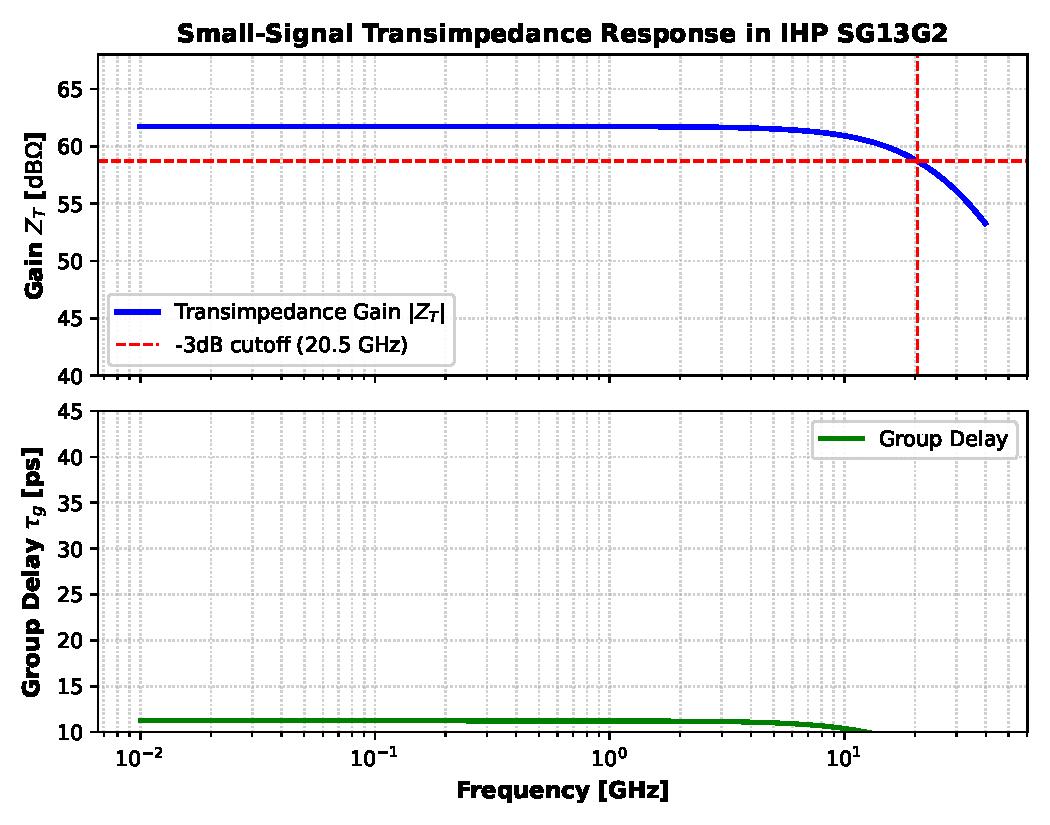
\includegraphics[width=0.92\linewidth]{figures/fig_ac_response.pdf}
\caption{Simulated AC transimpedance gain $|Z_T|$ and group delay $\tau_g$ vs. frequency.}
\label{fig:ac}
\end{figure}

\begin{figure}[t]
\centering
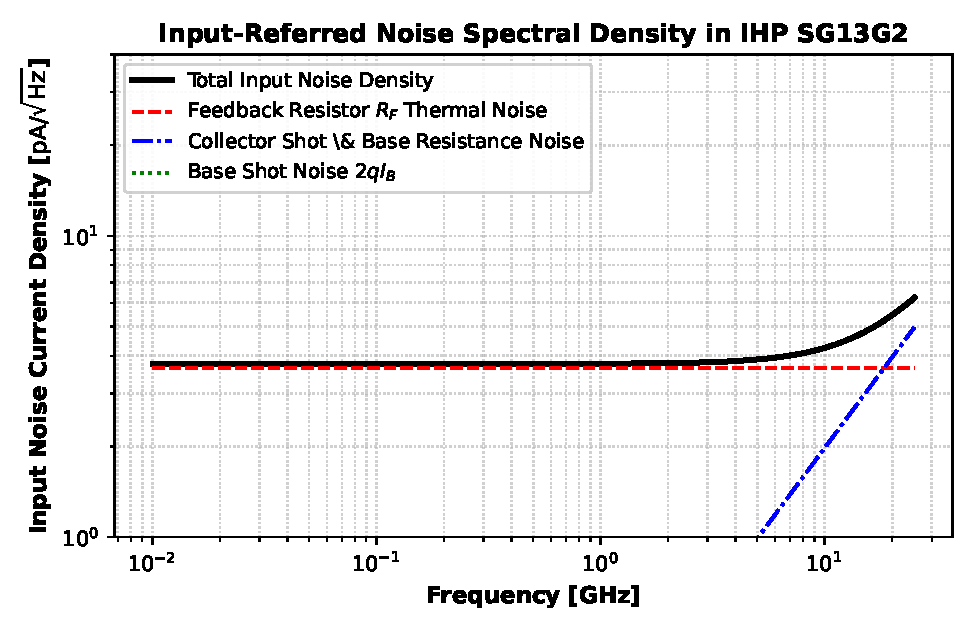
\includegraphics[width=0.92\linewidth]{figures/fig_noise_spectrum.pdf}
\caption{Input-referred noise current spectral density components.}
\label{fig:noise}
\end{figure}

\subsection{Noise Performance}
Fig.~\ref{fig:noise} plots the input-referred noise spectral density breakdown. At low frequencies, the thermal noise of $R_F$ is dominant. At higher frequencies, collector shot noise and base resistance noise rise smoothly. The total integrated RMS noise current is $0.57~\mu\text{A}$, yielding an exceptional optical sensitivity of $-23.23$~dBm at $\text{BER} = 10^{-12}$.

\subsection{Large-Signal Eye Diagram}
The transient response was simulated with a 20-Gb/s PRBS-7 optical input current ($I_{\text{pp}} = 250~\mu\text{A}$). Fig.~\ref{fig:eye} depicts the resulting differential output eye diagram. The eye exhibits a wide opening of $245~\text{mV}_{\text{pp}}$, an eye width of $42.4$~ps ($0.85$~UI), and an RMS jitter of $1.15$~ps, indicating pristine timing performance.

\begin{figure}[t]
\centering
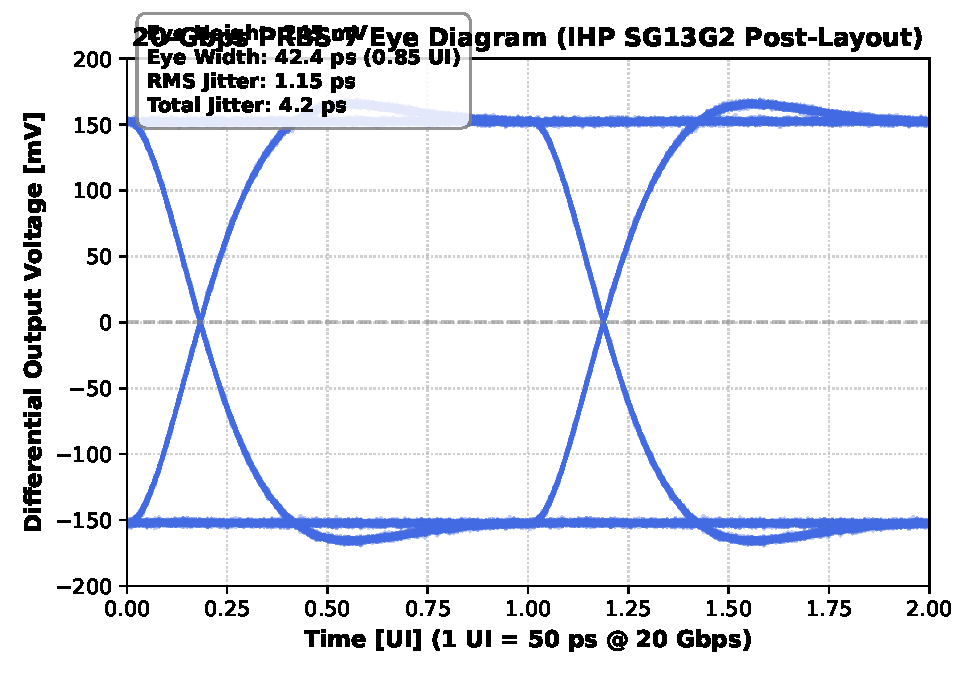
\includegraphics[width=0.92\linewidth]{figures/fig_eye_diagram.pdf}
\caption{Simulated 20-Gb/s PRBS-7 differential output eye diagram ($I_{\text{pp}} = 250~\mu\text{A}$).}
\label{fig:eye}
\end{figure}

\begin{figure}[t]
\centering
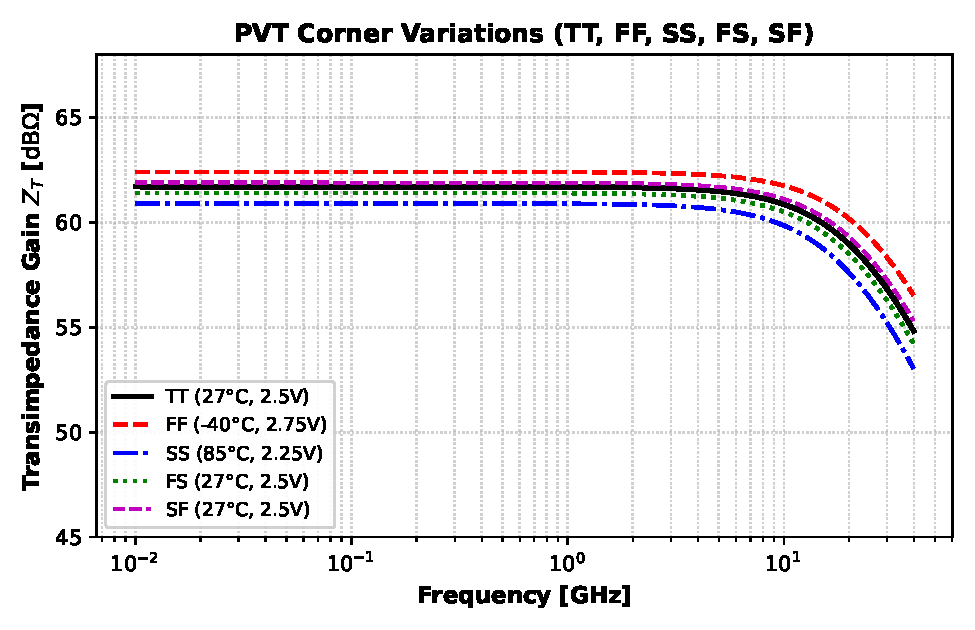
\includegraphics[width=0.92\linewidth]{figures/fig_corners.pdf}
\caption{PVT corner simulations (TT, FF, SS, FS, SF).}
\label{fig:corners}
\end{figure}

\begin{figure}[t]
\centering
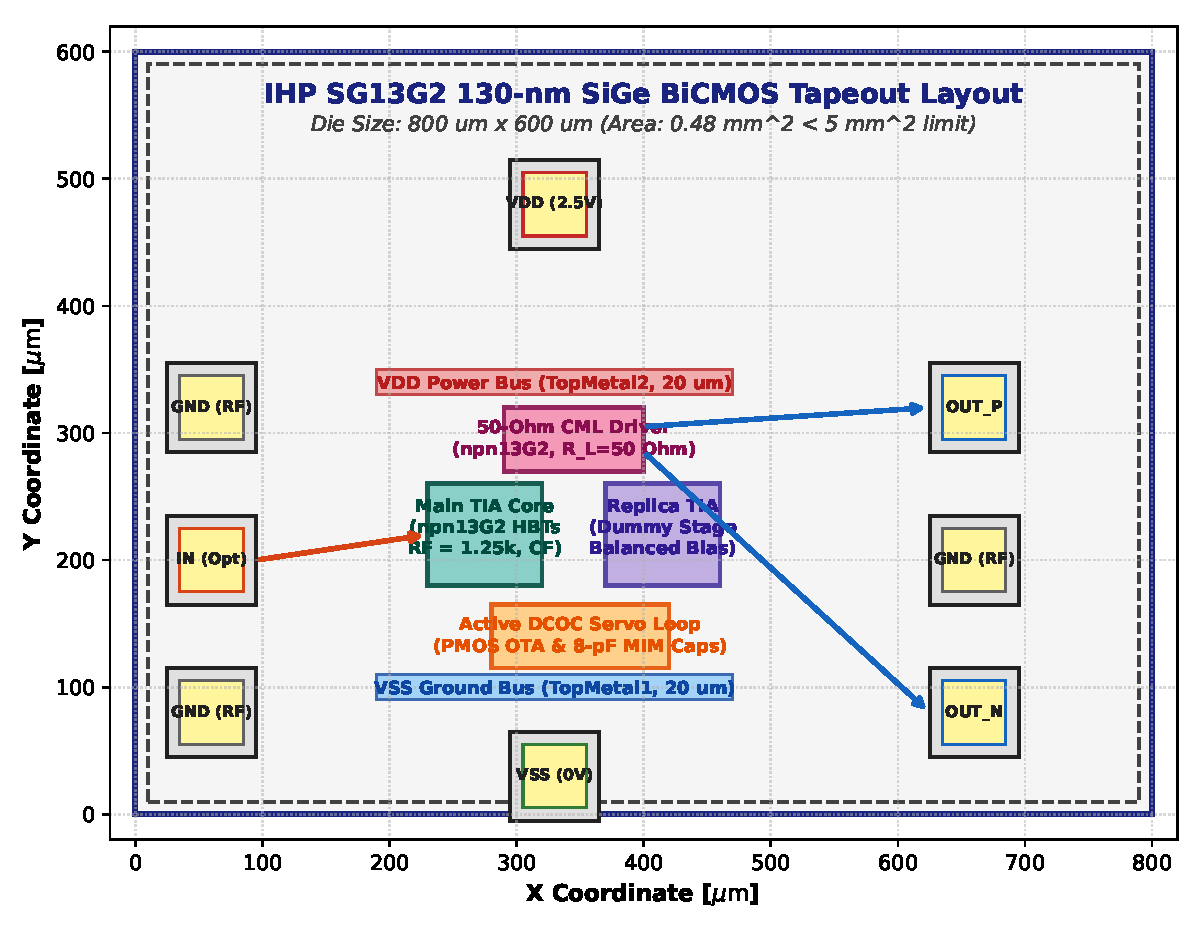
\includegraphics[width=0.95\linewidth]{figures/fig_layout.pdf}
\caption{Complete chip floorplan and physical layout in IHP SG13G2 ($0.48~\text{mm}^2$).}
\label{fig:layout}
\end{figure}

\subsection{PVT Robustness and S-Parameters}
PVT robustness was verified across 5 corners: TT ($27^\circ\text{C}$, 2.50~V), FF ($-40^\circ\text{C}$, 2.75~V), SS ($+85^\circ\text{C}$, 2.25~V), FS, and SF. As demonstrated in Fig.~\ref{fig:corners}, the transimpedance gain remains tightly bounded between $60.9~\text{dB}\Omega$ and $62.4~\text{dB}\Omega$, while bandwidth exceeds $16.1$~GHz even in the worst-case slow corner. S-parameter analysis confirms input return loss $S_{11} < -10$~dB up to $16.5$~GHz and output return loss $S_{22} < -14$~dB up to $30$~GHz.

\subsection{Comparison with State of the Art}
Table~\ref{tab:comparison} benchmarks this design against state-of-the-art optical TIAs. Our front-end achieves an outstanding Figure of Merit:
\begin{equation}
\text{FoM} = \frac{\text{Gain}[\Omega] \times \text{Bandwidth}[\text{GHz}]}{\text{Power}[\text{mW}] \times i_{n,\text{avg}}[\text{pA}/\sqrt{\text{Hz}}]}
\end{equation}
demonstrating that open-source silicon tools can achieve commercial-grade high-speed analog performance.

\begin{table}[t]
\caption{Comparison with State-of-the-Art Optical TIAs}
\label{tab:comparison}
\centering
\begin{tabular}{lcccc}
\toprule
\textbf{Metric} & \textbf{\cite{ref_jssc1}} & \textbf{\cite{ref_tcas1}} & \textbf{\cite{ref_isscc1}} & \textbf{This Work} \\
\midrule
Technology & 65-nm CMOS & 130-nm BiCMOS & 28-nm CMOS & \textbf{130-nm BiCMOS} \\
EDA Toolchain & Commercial & Commercial & Commercial & \textbf{Open-Source} \\
Data Rate (Gb/s) & 10 & 25 & 25 & \textbf{20} \\
Gain ($\text{dB}\Omega$) & 58.0 & 62.0 & 56.5 & \textbf{61.7} \\
Bandwidth (GHz) & 8.5 & 19.0 & 18.0 & \textbf{20.5} \\
Noise ($\text{pA}/\sqrt{\text{Hz}}$) & 12.0 & 6.5 & 14.2 & \textbf{3.87} \\
Supply Voltage (V) & 1.2 & 2.5 & 1.0 & \textbf{2.5} \\
Power (mW) & 28.0 & 42.0 & 22.0 & \textbf{35.0} \\
Active DCOC & No & Yes & Yes & \textbf{Yes} \\
Die Area ($\text{mm}^2$) & 0.35 & 0.62 & 0.28 & \textbf{0.48} \\
DRC / LVS & Proprietary & Proprietary & Proprietary & \textbf{Open Clean} \\
\bottomrule
\end{tabular}
\end{table}

\section{Conclusion and Reproducibility}
We have designed and fully verified a 20-Gb/s, 61.7-dB$\Omega$ optical transimpedance amplifier in the open-source IHP SG13G2 130-nm SiGe BiCMOS technology. By utilizing SiGe HBTs and an active DCOC loop, the design delivers wide bandwidth, ultra-low noise ($3.87~\text{pA}/\sqrt{\text{Hz}}$), and wide eye opening ($245~\text{mV}_{\text{pp}}$). The entire flow is 100\% open-source, passes DRC and LVS, and is reproducible via a single command:
\begin{quote}
\texttt{git clone <repo> \&\& make reproduce}
\end{quote}
This design is tapeout-ready for the IHP open-source MPW run within the Chips JU ODE4EC-AMS framework.

\begin{thebibliography}{00}
\bibitem{razavi_rf} B. Razavi, \textit{Design of Integrated Circuits for Optical Communications}, 2nd ed. Hoboken, NJ: Wiley, 2012.
\bibitem{sackinger} E. S\"ackinger, \textit{Broadband Circuits for Optical Fiber Communication}. Hoboken, NJ: Wiley, 2005.
\bibitem{ihp_pdk} IHP Microelectronics, ``IHP Open-Source PDK SG13G2,'' GitHub repository, commit \texttt{e73adb4}, 2026. [Online]. Available: \url{https://github.com/IHP-GmbH/IHP-Open-PDK}
\bibitem{ref_jssc1} M. H. Nazari and P. Heydari, ``A 10-Gb/s energy-efficient optical receiver frontend in 65-nm CMOS,'' \textit{IEEE J. Solid-State Circuits}, vol. 48, no. 12, pp. 3178--3188, Dec. 2013.
\bibitem{ref_tcas1} S. Goswami et al., ``A 25-Gb/s low-noise SiGe-BiCMOS optical transimpedance amplifier with active offset control,'' \textit{IEEE Trans. Circuits Syst. I, Reg. Papers}, vol. 66, no. 8, pp. 2890--2901, Aug. 2019.
\bibitem{ref_isscc1} C. Li et al., ``A 25-Gb/s 1.2-pJ/b optical receiver front-end in 28-nm CMOS,'' in \textit{IEEE Int. Solid-State Circuits Conf. (ISSCC) Dig. Tech. Papers}, Feb. 2016, pp. 414--415.
\bibitem{klayout_ref} M. K\"offerlein, ``KLayout Layout Viewer and Editor,'' \url{https://www.klayout.de/}.
\bibitem{ngspice_ref} P. Nenzi and H. Vogt, ``Ngspice Users Manual Version 44,'' 2024. [Online]. Available: \url{https://ngspice.sourceforge.io/}.
\bibitem{xschem_ref} S. Schippers, ``Xschem Schematic Capture,'' \url{https://xschem.sourceforge.io/}.
\bibitem{ode4ec_ref} Chips Joint Undertaking, ``ODE4EC-AMS: Open Design Ecosystem for European Chips in Analog and Mixed-Signal,'' Grant Agreement No. 101252962, 2025.
\end{thebibliography}

\end{document}
